\documentclass[paper=a4, fontsize=11pt]{scrartcl} % A4 paper and 11pt font size
\usepackage[section]{placeins}
\usepackage[T1]{fontenc}
\usepackage[polish]{babel}
\usepackage[utf8]{inputenc}
\usepackage{lmodern}
\selectlanguage{polish}
\usepackage{amsmath,amsfonts,amsthm} % Math packages
\usepackage{listings}   
\usepackage{enumerate}
\usepackage{tikz}
\usepackage{circuitikz}
\usepackage{graphicx}
\usepackage{dblfloatfix}
\usepackage{caption}
\usepackage{longtable}
\usepackage{chngcntr}
\usepackage{sectsty} % Allows customizing section commands
\usepackage{float}
\allsectionsfont{\centering \normalfont\scshape} % Make all sections centered, the default font and small caps
\setlength\parindent{0pt} % Removes all indentation from paragraphs - comment this line for an assignment with lots of text
\usepackage[colorinlistoftodos]{todonotes}
\usepackage[colorlinks=true, allcolors=blue]{hyperref}
\usepackage{ltablex}

%----------------------------------------------------------------------------------------
%	TITLE SECTION
%----------------------------------------------------------------------------------------

\newcommand{\horrule}[1]{\rule{\linewidth}{#1}} % Create horizontal rule command with 1 argument of height

\title{	
\normalfont \normalsize 
\textsc{Politechnika Warszawska, WEiTI} \\ [25pt] % Your university, school and/or department name(s)
\horrule{0.5pt} \\[0.4cm] % Thin top horizontal rule
\huge pRoman - process manager \\
\large Projekt TIN. Dokumentacja wstępna
 \\ % The assignment title
\horrule{2pt} \\[0.5cm] % Thick bottom horizontal rule
}

\author{Damian Bułak\\ Michał Sypetkowski\\ Marcin Waszak\\ Ahata Valiukevich} % Your name

\date{\normalsize\today} % Today's date or a custom date

%----------------------------------------------------------------------------------------
%
%----------------------------------------------------------------------------------------

\begin{document}

\maketitle % Print the title


\section*{Treść zadania}

W sieci jest zbiór zarządzanych węzłów, serwer zarządzający i stacja konsoli administratora. W węzłach pracują agenty zarządzające. Agent zarządzający może: załadować kod nowego procesu, usunąć kod procesu, uruchomić/zatrzymać/wznowić/zabić dany proces zgodnie z harmonogramem, wznowić proces nie raportujący swej żywotności, podać dane statystyczne serwerowi. System umożliwia administratorowi zarządzanie rozproszonymi procesami. System komunikacji powinien móc pracować w przestrzeni adresów \textit{IPv4} i \textit{IPv6}. Ponadto należy zaprojektować moduł do \textit{Wireshark} umożliwiający wyświetlanie i analizę zdefiniowanych komunikatów. 


\section*{Przyjęte założenia funkcjonalne i niefunkcjonalne}

\subsection*{Założenia funkcjonalne}
Implementowany system ma umożliwiać: 
\begin{itemize}
\item wysyłanie obrazu procesu
\item usuwanie obrazu procesu
\item wznawianie  procesu nie raportującego swej żywotności 
\item podawanie danych statystycznych serwerowi
\item uruchamianie danego procesu zgodnie z harmonogramem
\item zatrzymywanie danego procesu zgodnie z harmonogramem
\item wznawianie danego procesu zgodnie z harmonogramem
\item zabijanie danego procesu zgodnie z harmonogramem
\end{itemize}

\subsection*{Założenia niefunkcjonalne}
\begin{itemize}
\item niezawodność komunikacji dzięki użyciu protokołu TCP
\item funkcja watchdoga chroniącego przed zawieszaniu się agenta
\item intuicyjna obsługa dzięki zastosowaniu poleceń z poziomu konsoli
\end{itemize}


\section*{Podstawowe przypadki użycia}
Administrator - użytkownik zalogowany do konsoli administratorskiej
\begin{longtable}{ |m{4.5cm}|m{3cm}|m{7.5cm}|}
 \caption{Podstawowe przypadki użycia}\\
 \hline
NAZWA & AKTORZY & OPIS \\
 \hline
 \endfirsthead
 \multicolumn{3}{c}%
{\tablename\ \thetable\ -- \textit{Kontynuacja z poprzedniej strony}} \\
\hline
 NAZWA & AKTORZY & OPIS\\
 \hline
 \endhead
 \hline \multicolumn{3}{r}{\textit{Kontynuacja na następnej stronie}} \\
 \endfoot
 \hline
 \endlastfoot
 Wysłanie obrazu procesu & Administrator & 
\begin{enumerate}
\item Administrator wybiera proces do załadowania.
\item Proces zostaje załadowany do systemu.
\end{enumerate} \\
 \hline
Przeglądanie listy procesów & Administrator & 
\begin{enumerate}
\item Administratorowi prezentowana jest lista załadowanych procesów.
\item Obok każdego procesu administrator może zobaczyć stan procesu (uruchomiony bądź nie), jak i podstawowe informacje o procesie.
\end{enumerate}\\
 \hline
Usuwanie obrazu procesu & Administrator & 
\begin{enumerate}
\item $[$ Przeglądanie listy procesów $]$
\item Administrator usuwa wybrany z listy proces poleceniem \textit{‘Usuń’}.
\end{enumerate} \\
 \hline
Uruchomienie procesu & Administrator & 
\begin{enumerate}
\item $[$ Przeglądanie listy procesów $]$
\item Administrator wybiera z listy proces i uruchamia go poleceniem \textit{‘Uruchom’}.
\item Następuje przetwarzanie procesu (opis w architekturze systemu). Administrator może zobaczyć postęp przetwarzania procesu w postaci procent zakończenia.
\item Po zakończeniu przetwarzania administrator widzi rezultat przetwarzania.
\end{enumerate} \\
 \hline
Zatrzymanie uruchomionego procesu & Administrator & 
\begin{enumerate}
\item $[$ Przeglądanie listy procesów $]$
\item Administrator wybiera z listy uruchomiony proces.
\item Administrator zatrzymuje proces poleceniem \textit{‘Zatrzymaj’}.
\end{enumerate} \\
 \hline
Planowanie czasu uruchomienia procesu & Administrator & 
\begin{enumerate}
\item $[$ Przeglądanie listy procesów $]$
\item Administrator edytuje czas wykonania procesu po wpisaniu polecenia \textit{‘Edytuj’}.
\end{enumerate} \\
 \hline
Podgląd harmonogramu procesów & Administrator & 
\begin{enumerate}
\item Administrator przegląda tabelaryczny harmonogram załadowanych procesów.
\end{enumerate} \\
 \hline
Podgląd danych statystycznych & Administrator & 
\begin{enumerate}
\item Administrator przegląda dane statystyczne z informacjami o załadowanych, uruchomionych, zatrzymanych procesach oraz o obciążeniu poszczególnych węzłów.
\end{enumerate} \\
 \hline
\end{longtable}

\section*{Wybrane środowisko sprzętowo-programowe} 
\begin{enumerate}
\item System operacyjny: \textit{\textbf{GNU/Linux}}.
\item Język: \textit{\textbf{C++}}.
\item Biblioteki: STL, boost/filesystem, boost/process, BSD Sockets API.
\item Testowanie: boost/test.
\item Debugowanie: wireshark.
\item Budowanie: cmake
\end{enumerate}

\section*{Architektura rozwiązania}
\begin{figure}[H]
    \centering
    \def\svgwidth{0.5\columnwidth}
    \input{image.pdf_tex}
    \caption{Ilustracja systemu}\label{visina8}
\end{figure}
\textbf{\textit{Węzeł worker}} - maszyna, która wykonuje procesy. Bezpośrednia kontrola procesów jest sprawowana przez procesy sieciowe klasy worker.\\
\textbf{\textit{Proces klasy worker}}- specjalny proces sieciowy na maszynach węzłów worker. Jego zadaniem jest zarządzanie procesami na tych maszynach według rozkazów serwera zarządzającego.\\
\textbf{\textit{Watchdog}} - specjalny proces obok procesu workera. Stanowi zabezpieczenie przed skutkami zawieszenia procesu workera. \\
\textbf{\textit{Serwer zarządzający}} - maszyna, która wysyła rozkazy do agentów maszyn węzłowych. Może przeprowadzać zaplanowane wcześniej czynności. Serwer posiada proces sieciowy klasy server.\\
\textbf{\textit{Proces klasy server}} - oczekuje na połączenia od węzłów worker i terminali administratora.\\
\textbf{\textit{Terminal administratora}} - maszyna, dzięki której administrator ma możliwość zarządzać procesami na maszynach węzłowych. Każdy taki terminal posiada proces sieciowy klasy administrator.\\

Planowane aplikacje sieciowe do wykonania:
\begin{itemize}
\item aplikacja klasy worker
\item aplikacja klasy server
\item aplikacja klasy administrator
\end{itemize}

\section*{API modułów stanowiących bloki funkcjonalne}
\begin{figure}[H]
	\centering
	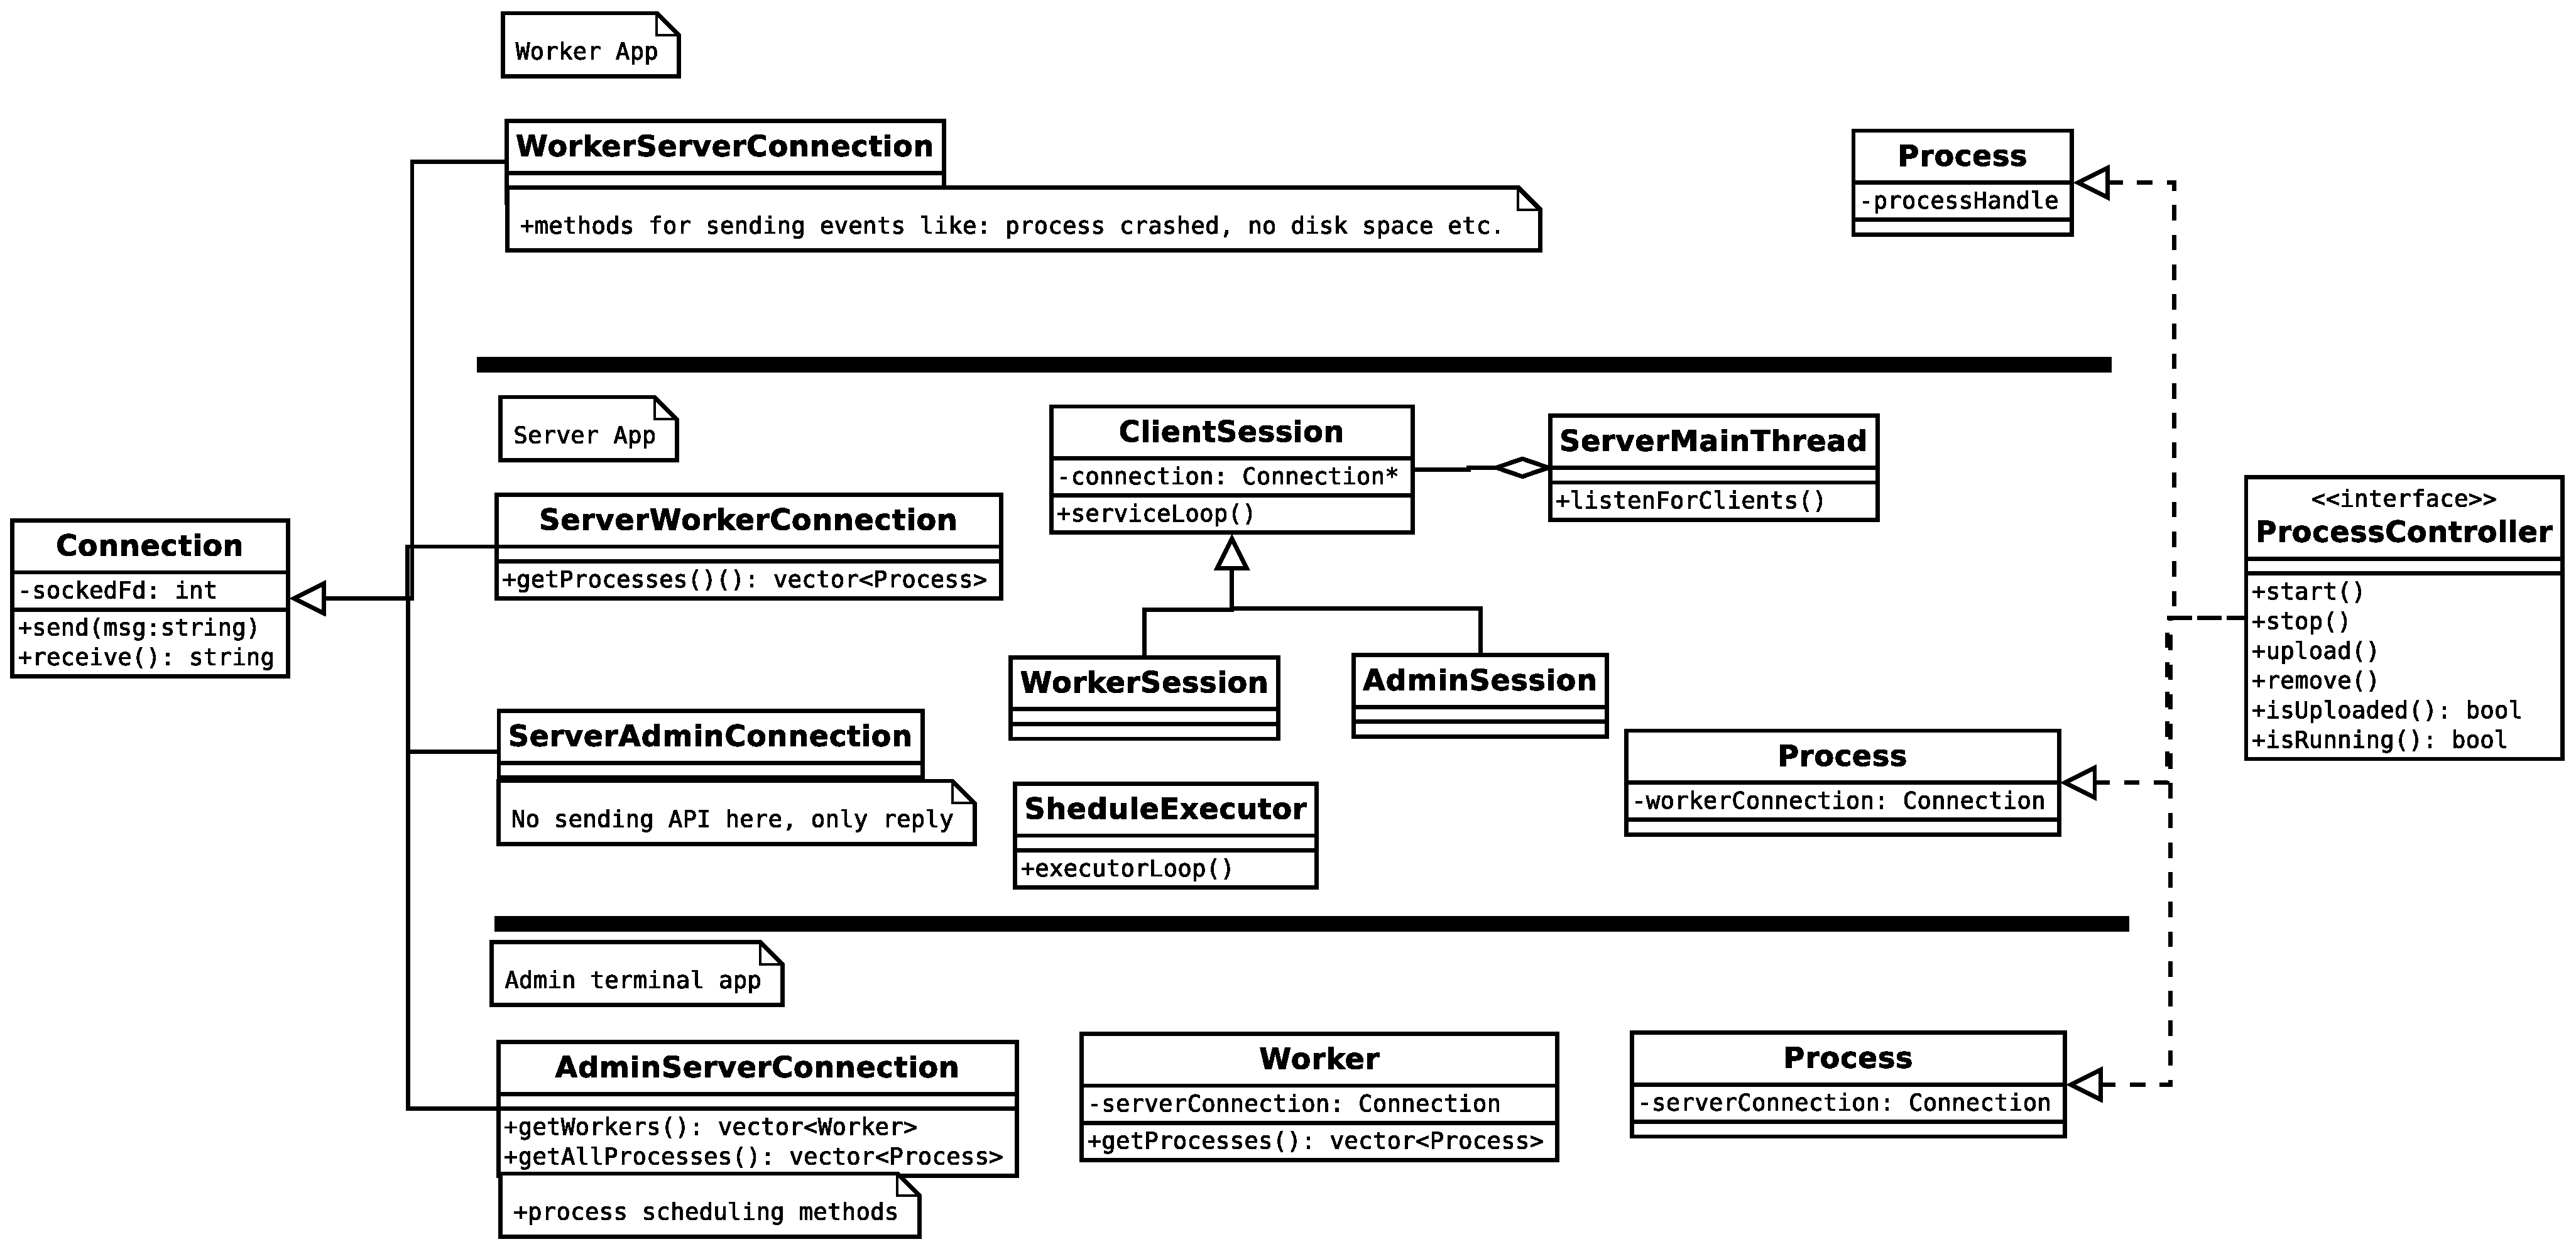
\includegraphics[scale=.25]{tin.eps}
	\caption{Wstępny diagram klas}
\end{figure}

\section*{Sposób testowania} 
Planujemy użyć testów jednostkowych w poszczególnych aplikacjach naszego projektu, żeby sprawdzić poprawność działania osobnych części całego systemu. Poza testami jednostkowymi napisane będą również testy integracyjne. Przewidujemy rownież testowanie ręczne. Scenariusze testów akceptacyjnych są przedstawione poniżej.

\newpage
\section*{Scenariusze testów akceptacyjnych}
Testy akceptacyjne będą polegały na wykonywaniu różnych scenariuszy użycia.

\begin{longtable}{ |m{4.0cm}|m{5.5cm}|m{6.0cm}|}
 \caption{Przykładowe scenariusze testów akceptacyjnych}\\
 \hline
CEL TESTU & OPIS PRZEBIEGU & OCZEKIWANY WYNIK \\
 \hline
 \endfirsthead
 \multicolumn{3}{c}%
{\tablename\ \thetable\ -- \textit{Kontynuacja z poprzedniej strony}} \\
\hline
 CEL TESTU & OPIS PRZEBIEGU & OCZEKIWANY WYNIK\\
 \hline
 \endhead
 \hline \multicolumn{3}{r}{\textit{Kontynuacja na następnej stronie}} \\
 \endfoot
 \hline
 \endlastfoot
 Usuwanie obrazu procesu & Administrator przegląda listę procesów. Wpisuje polecenie do usunięcia procesu oraz jego id. & 
Jeśli podane id istnieje, obraz procesu zostanie usunięty, w przeciwnym przypadku pojawi się komunikat o braku danego procesu. \\
 \hline
 Zatrzymanie uruchomionego procesu & Administrator wpisuje polecenie zatrzymania procesu. & Administrator otrzymuje informację o zatrzymaniu procesu.Proces jest widoczny na liście procesów jako załadowany (nie uruchomiony). Jeśli proces nie został jeszcze uruchomiony administrator otrzymuje informację o błędzie. \\
 \hline
 Załadowanie obrazu procesu & Administrator wpisuje polecenie załadowania nowego obrazu procesu. & Informacja o stanie załadowania procesu - sukces lub nieudane załadowanie, wraz ze wskazaniem przyczyn niepowodzenia w wykonaniu polecenia. \\
 \hline
 Podgląd harmonogramu procesów & Administrator wpisuje polecenie przeglądu procesów. & Wyświetlona lista procesów wraz z ich planowanymi czasami uruchomienia. \\
 \hline
 Podgląd danych statystycznych & Administrator wpisuje polecenie służące do podglądu danych statystycznych serwera. & Wyświetlone zostaną informacje o obciążeniu węzłów, liczbie uruchomionych procesów, liczbie załadowanych procesów etc.\\
  \hline
\end{longtable}
\section*{Podział prac w zespole}
\textbf{Damian:} projekt architektury \\
\textbf{Michał:} projekt architektury \\
\textbf{Agata:} projekt architektury, dokumentacja, testowanie, moduł Wireshark \\
\textbf{Marcin:} team-leader, projekt architektury \\

Powyższy podział jest zgrubny. Bowiem szczegółowe przydzielanie prac zorganizowane zostało za pomocą systemu tasków na platformie GitHub.

\section*{Harmonogram prac}
\begin{itemize}
\item \textbf{19.04} - oddanie dokumentacji wstępnej. 
\item \textbf{30.04} - szkielet programów: serwera, workera oraz administratora;  rozpoczęte prace nad skryptami testującymi. 
\item \textbf{8.05} - konsultacje \#1: projekt z w pełni działającą komunikacją między administratorem a serwerem (nawiązywanie połączenia, działający mechanizm przesyłania pakietów i poleceń). 
\item \textbf{22.05} - konsultacje \#2: działający i prawie skończony projekt, z ewentualnymi błędami niewpływającymi istotnie na działanie programu, rozpoczęcie pracy nad końcową dokumentacją poprojektową. 
\item \textbf{31.05} - oddanie projektu.
\end{itemize}

\section*{Adres projektu na serwerze kontroli wersji}
\url{https://github.com/marcin-waszak/DistributedProcesses}  \\

W zakadce \textit{Issues} można przeglądać informacje o przydzielanych przez Marcina zadaniach: 
\begin{itemize}
\item dla kogo zostało przydzielone
\item kiedy zostało utworzone
\item na jakim etapie realizacji obecnie jest
\end{itemize}
\end{document}